\documentclass[10pt,preprint,blind,clearpagebib]{sigplanconf}

\usepackage{listings}
\usepackage{enumitem}
\usepackage[hyphens]{url}
\usepackage[svgnames]{xcolor}
\definecolor{lcl}{RGB}{140,0,100}
\usepackage[colorlinks=true,breaklinks,draft=false]{hyperref}
\hypersetup{urlcolor=lcl,linkcolor=lcl,citecolor=lcl}
\newcommand{\doi}[1]{doi:~\href{http://dx.doi.org/#1}{\Hurl{#1}}}
\usepackage{amssymb}
\usepackage{multicol}
\usepackage{xcolor}
\usepackage{graphicx}
\usepackage[fleqn]{amsmath}
\usepackage{graphics} 
\usepackage{stmaryrd}
\usepackage{amsthm}
\usepackage{ftnright}
\usepackage[T1]{fontenc}
\usepackage{semantic}
\usepackage{enumitem}
\usepackage[hang,flushmargin]{footmisc} 
\usepackage[notquote]{hanging}
\usepackage{flushend}

% =================================================================================================

% TODO: Discuss 'stability' of the inference (minor change in schema does not cause dramatic cahnges)
% TODO: Say that variant is a last-resort thing
% TODO: Practical evaluation (lots of downloads, lots of Github - how often people customize samples?)
% TODO: Explain why we need option type (because T + null is a variant)
% TODO: In the PLDI version, we delete all the unnecessary runtime conversions
% but we should say that those happen for practical reasons (e.g. float -> int, or anyhing to string)

\urlstyle{sf}

\makeatletter
\renewcommand{\@makefntext}[1]{%
  \parindent 1em%
  \raggedright
  \begin{hangparas}{0.8em}{1}
  \noindent {$^{\@thefnmark}$~#1}
  \end{hangparas}
}
\makeatother

\newcommand{\langl}{\begin{picture}(4.5,7)
\put(1.1,2.5){\rotatebox{60}{\line(1,0){5.5}}}
\put(1.1,2.5){\rotatebox{300}{\line(1,0){5.5}}}
\end{picture}}
\newcommand{\rangl}{\begin{picture}(4.5,7)
\put(.9,2.5){\rotatebox{120}{\line(1,0){5.5}}}
\put(.9,2.5){\rotatebox{240}{\line(1,0){5.5}}}
\end{picture}}

\newcommand{\lang}{\begin{picture}(5,7)
\put(1.1,2.5){\rotatebox{45}{\line(1,0){6.0}}}
\put(1.1,2.5){\rotatebox{315}{\line(1,0){6.0}}}
\end{picture}}
\newcommand{\rang}{\begin{picture}(5,7)
\put(.1,2.5){\rotatebox{135}{\line(1,0){6.0}}}
\put(.1,2.5){\rotatebox{225}{\line(1,0){6.0}}}
\end{picture}} 

\newcommand{\llangl}{\langl\hspace{-0.35em}\langl}
\newcommand{\rrangl}{\rangl\hspace{-0.35em}\rangl}

\definecolor{cmtclr}{rgb}{0.0,0.6,0.0}
\definecolor{numclr}{rgb}{0.0,0.4,0.0}
\definecolor{kvdclr}{rgb}{0.0,0.0,0.6}
\definecolor{strclr}{rgb}{0.5,0.1,0.0}
\definecolor{prepclr}{rgb}{0.0,0.0,0.0}

\newcommand{\kvd}[1]{\textnormal{\textcolor{kvdclr}{\sffamily #1}}}
\newcommand{\num}[1]{\textnormal{\textcolor{numclr}{\sffamily #1}}}
\newcommand{\str}[1]{\textnormal{\textcolor{strclr}{\sffamily "#1"}}}
\newcommand{\strf}[1]{\textnormal{\textcolor{strclr}{\sffamily #1}}}
\newcommand{\ident}[1]{\textnormal{\sffamily #1}}
\newcommand{\lident}[1]{\textnormal{\sffamily\`{}\hspace{-0.25em}\`{}\hspace{-0.1em}#1\`{}\hspace{-0.25em}\`{}}}
\newcommand{\cmt}[1]{\textit{\sffamily\textcolor{cmtclr}{#1}}}

\newcommand{\lsep}[0]{\;\; | \;\;}
\newcommand{\narrow}[1]{\hspace{-0.7em} #1 \hspace{-0.7em}}

\newcommand{\tsep}[0]{\; \triangledown \;}
\newcommand{\tytag}{\ident{tag}}
\newcommand{\dropopt}[1]{\lfloor#1\rfloor}
\newcommand{\addopt}[1]{\lceil#1\rceil}
\newcommand{\tytagof}{\ident{tagof}}

\newcommand{\reduce}{\rightsquigarrow}

\newcommand{\sem}[1]{\llbracket #1 \rrbracket}
\newcommand{\semalt}[1]{S(#1)}

\newtheorem{definition}{Definition}
\newtheorem{theorem}{Theorem}
\newtheorem{corollary}[theorem]{Corollary}
\newtheorem{lemma}[theorem]{Lemma}

% =================================================================================================

\begin{document}

\special{papersize=8.5in,11in}
\setlength{\pdfpageheight}{\paperheight}
\setlength{\pdfpagewidth}{\paperwidth}
\conferenceinfo{CONF 'yy}{Month d--d, 20yy, City, ST, Country} 
\copyrightyear{20yy} 
\copyrightdata{978-1-nnnn-nnnn-n/yy/mm} 
%\doi{nnnnnnn.nnnnnnn}

%\titlebanner{Unpublished draft, March 2015}        % These are ignored unless
%\preprintfooter{short description of paper}        % 'preprint' option specified.

\title{Types from data: \textnormal{Making structured data first-class citizens in F\#}}
%\subtitle{Subtitle Text, if any}

\authorinfo{Tomas Petricek}
           {University of Cambridge}
           {tomas@tomasp.net}
\authorinfo{Gustavo Guerra}
           {Microsoft Corporation, London}
           {gustavo@codebeside.org}
\authorinfo{Don Syme}
           {Microsoft Research, Cambridge}
           {dsyme@microsoft.com}
\maketitle

% =================================================================================================

\begin{abstract}
Most modern applications interact with external services and access data in structured formats such 
as XML, JSON and CSV. Static type systems do not understand such formats, often making data access
more cumbersome. Should we give up and leave the messy world of external data to dynamic typing 
and runtime checks? Of course, not!

In this paper, we integrate external structured data into F\# programming. As most real-world data
does not come with an explicit schema, we develop a shape inference algorithm that infers a shape from 
representative sample documents and transforms the shape into F\# types using type providers.
We present a formalization and a relative type soundness theorem for a simplified version of this process.

Our library significantly reduces the amount of data access code and it provides additional 
safety guarantees when contrasted with the widely used weakly typed techniques.
\end{abstract}

\category{D.3.3}{Programming Languages}{Language Constructs and Features }
\keywords F\#, Type Providers, Inference, JSON, XML



% =================================================================================================
%
%   ###                                                                       
%    #  #    # ##### #####   ####  #####  #    #  ####  ##### #  ####  #    # 
%    #  ##   #   #   #    # #    # #    # #    # #    #   #   # #    # ##   # 
%    #  # #  #   #   #    # #    # #    # #    # #        #   # #    # # #  # 
%    #  #  # #   #   #####  #    # #    # #    # #        #   # #    # #  # # 
%    #  #   ##   #   #   #  #    # #    # #    # #    #   #   # #    # #   ## 
%   ### #    #   #   #    #  ####  #####   ####   ####    #   #  ####  #    # 
%
% =================================================================================================

\section{Introduction}
\label{sec:introduction}

Applications for social networks, finding tomorrow's weather or searching train schedules
all communicate with external services. Increasingly, these services provide end-points that return 
data as CSV, XML or JSON. Most such services do not come with an explicit schema. At best, the 
documentation provides sample responses for typical requests.

For example, \url{http://openweathermap.org/current} documents an end-point to get the current 
weather with one example. Using standard libraries, we might call it as:

\noindent
\begin{equation*}
\begin{array}{l}
 \kvd{let}~\ident{doc}=\ident{Http.Request}(\str{http://api.owm.org/?q=NYC}) \\
 \kvd{match}~\ident{JsonValue.Parse}(\ident{doc})~\kvd{with} \\
 |~\ident{Record}(\ident{root})\rightarrow \\
 \quad \kvd{match}~\ident{Map.find}~\str{main}~\ident{root}~\kvd{with} \\
 \quad |~\ident{Record}(\ident{main})\rightarrow \\
 \quad \quad \kvd{match}~\ident{Map.find}~\str{temp}~\ident{main}~\kvd{with} \\
 \quad \quad |~\ident{Number}(\ident{num})\rightarrow \ident{printfn}~\str{Lovely \%f!}~\ident{num} \\
 \quad \quad |~\_\rightarrow \ident{failwith}~\str{Incorrect format} \\
 \quad |~\_\rightarrow \ident{failwith}~\str{Incorrect format} \\
 |~\_\rightarrow \ident{failwith}~\str{Incorrect format} 
\end{array}
\end{equation*}
%
The code assumes that the response has a particular shape described in the documentation. The
root node must be a record with a \str{main} field, which has to be another record containing
a numerical \str{temp} field. When the shape is different, the code simply fails with an exception. 
While not immediately unsound, the code is manifestly prone to errors if strings are misspelled 
or incorrect shape assumed.

Using the JSON type provider from F\# Data, we can write code with exactly the 
same functionality in two lines:
%
\vspace{-0.1em}
\begin{equation*}
\begin{array}{l}
 \kvd{type}~\ident{W} = \ident{JsonProvider}\langl\str{http://api.owm.org/?q=NYC}\rangl \\[0.1em]
 \ident{printfn}~\str{Lovely \%f!}~(\ident{W.GetSample().Main.Temp})
\end{array}
\end{equation*}
%
$\ident{JsonProvider}\langl\str{...}\rangl$ invokes a type provider \cite{fsharp-typeprov} at 
compile-time with the URL as a sample. The type provider infers the structure of the response
and provides a type with a \ident{GetSample} method that returns a parsed JSON with nested
properties \ident{Main.Temp}, returning the temperature as a number.

In short, \emph{the types come from the sample data}. In our experience, this technique is 
both practical and surprisingly effective in achieving more sound information interchange 
in heterogeneous systems. Our contributions are as follows:

\begin{itemize}
\item We present F\# Data type providers for XML, CSV and JSON (\S\ref{sec:providers}) 
  and practical aspects of their implementation that contributed to their industrial 
  adoption (\S\ref{sec:impl}). 

\item We describe a predictable shape inference algorithm for structured data formats, 
  based on a \emph{preferred shape} relation, that underlies the type providers 
  (\S\ref{sec:inference}).

\item We give a formal model (\S\ref{sec:formal}) and use it to prove
  \emph{relativized type safety} for the type providers (\S\ref{sec:safety}).
\end{itemize}

\vspace{-0.1em}
\noindent
The supplementary screencast illustrates the practical developer experience using 
  F\# Data with JSON, XML and CSV.


% =================================================================================================
%
%   #######                                                                                  
%      #    #   # #####  ######    #####  #####   ####  #    # # #####  ###### #####   ####  
%      #     # #  #    # #         #    # #    # #    # #    # # #    # #      #    # #      
%      #      #   #    # #####     #    # #    # #    # #    # # #    # #####  #    #  ####  
%      #      #   #####  #         #####  #####  #    # #    # # #    # #      #####       # 
%      #      #   #      #         #      #   #  #    #  #  #  # #    # #      #   #  #    # 
%      #      #   #      ######    #      #    #  ####    ##   # #####  ###### #    #  ####  
%
% =================================================================================================

\section{Type providers for structured data}
\label{sec:providers}

We start with an informal overview that shows how F\# Data type providers simplify working with 
JSON and XML. We introduce the necessary aspects of F\# type providers along the way. The examples 
in this section illustrate the key design principles of the shape inference algorithm:

\begin{itemize}
\item The mechanism is predictable. The user directly works with the provided types and should 
  understand why a specific type was produced from a given sample.\footnote{In particular, we do 
  not use probabilistic methods where adding an additional sample could completely change the 
  shape of the type.}

\item The type providers prefer F\# object types with properties. This allows extensible 
  (open-world) data formats (\S\ref{sec:providers-xml}) and it interacts well with developer tooling
  (\S\ref{sec:providers-json}). 

\item The above also makes our techniques applicable to any language with nominal 
  object types (e.g.~variations of Java or C\# with a type provider mechanism added).

\item Finally, the we handle practical concerns including
  support for different numerical types, \kvd{null} and missing data.
\end{itemize}

% --------------------------------------------------------------------------------------------------

\subsection{Working with JSON documents}
\label{sec:providers-json}

The JSON format is a popular data exchange format based on 
JavaScript data structures. The following is the definition of \ident{JsonValue} 
used earlier (\S\ref{sec:introduction}) to represent JSON data:
%
\begin{equation*}
\begin{array}{l}
 \kvd{type}~\ident{JsonValue} = \\[0.1em]
 \quad|~ \ident{Number}~\kvd{of}~\ident{float} ~~~~|~ \ident{Boolean}~\kvd{of}~\ident{bool} \\[0.1em]
 \quad|~ \ident{String}~\kvd{of}~\ident{string} ~~~~~~ |~ \ident{Null} \\[0.1em]
 \quad|~ \ident{Record}~\kvd{of}~\ident{Map}\langl\ident{string}, \ident{JsonValue}\rangl \\[0.1em]
 \quad|~ \ident{Array}~\kvd{of}~\ident{JsonValue}[] \\[0.1em]
\end{array}
\end{equation*}
%
The earlier example used only a nested record containing a number. To demonstrate other 
aspects of the JSON type provider, we look at an example that also involves an array:
%
{\small{
\begin{verbatim}
  [ { "name":"Jan", "age":25 }, { "name":"Tomas" },
    { "name":"Alexander", "age":3.5 } ]
\end{verbatim}
}}
%
\noindent
The standard approach to print the names and ages would be to pattern match on the parsed 
\ident{JsonValue}, check that the top-level node is a \ident{Array} and iterate over the elements 
checking that each element is a \ident{Record} with certain properties. We would throw an exception 
for values of an incorrect shape. As before, the code would specify field names as strings, which 
is error prone and can not be statically checked.

Assuming \strf{people.json} is the above example and \ident{data} is a string containing
JSON of the same shape, we can write:
%
\begin{equation*}
\begin{array}{l}
 \kvd{type}~\ident{People}~=~\ident{JsonProvider}\langl\str{people.json}\rangl\hspace{1em} \\[0.6em]
 \kvd{for}~\ident{item}~\kvd{in}~\ident{People.Parse}(\ident{data})~\kvd{do}\\[0.1em]
 \quad\ident{printf}~\str{\%s }~\ident{item.Name}\\[0.1em]
 \quad\ident{Option.iter}~(\ident{printf}~\str{(\%f)})~\ident{item.Age}
\end{array}
\end{equation*}
%
In contrast to the earlier example, we now use a local file \strf{people.json} as a sample for 
the type inference, but then processes data from another source. The code achieves a similar 
simplicity as when using dynamically typed languages, but it is statically type-checked.

\paragraph{Type providers.}
The notation $\ident{JsonProvider}\langl\str{people.json}\rangl$ passes a \emph{static parameter} 
to the type provider. Static parameters are resolved at compile-time and have to be constant. 
The provider analyzes the sample and provides a type  \ident{People}. F\# editors also 
execute the type provider in the background at development-time and use the provided types 
in auto-completion on ``.'' and background type-checking.

The \ident{JsonProvider} uses a shape inference algorithm and provides
the following F\# types for the sample:
%
\begin{equation*}
\begin{array}{l}
 \kvd{type}~\ident{Entity}~=  \\
 \quad \kvd{member}~\ident{Name}~:~\ident{string} \\
 \quad \kvd{member}~\ident{Age}~:~\ident{option}\langl \ident{float}\rangl \\[0.5em]
 \kvd{type}~\ident{People}~=  \\
 \quad \kvd{member}~\ident{GetSample}~:~\ident{unit}~\rightarrow~\ident{Entity}[] \\
 \quad \kvd{member}~\ident{Parse}~:~\ident{string}~\rightarrow~\ident{Entity}[] \\
\end{array}
\end{equation*}
%
The type \ident{Entity} represents the person. The field \ident{Name} is available for all
sample values and is inferred as \ident{string}. The field \ident{Age} is marked as optional,
because the value is missing in one sample. The two age values are an integer $25$ and a 
float $3.5$ and so the common inferred type is \ident{float}.

The type \ident{People} has two methods for reading data. \ident{GetSample} parses the
sample used for the inference and \ident{Parse} parses a JSON string. This lets us read
data at runtime, provided that it has the same shape as the static sample.

\paragraph{Error handling.}
In addition to the structure of the types, the type provider also specifies what code should be 
executed at run-time in place of \ident{item.Name} and other operations. The runtime behaviour is 
the same as in the earlier hand-written sample (\S\ref{sec:introduction}) -- a member access 
throws an exception if data does not have the expected shape.

Informally, the safety property (\S\ref{sec:safety}) states that if the inputs are compatible
with one of the static samples (i.e.~the samples are representative), then no exceptions will 
occur. In other words, we cannot avoid all failures, but we can prevent some. Moreover, if 
\url{http://openweathermap.org} changes the shape of the response, the code in \S\ref{sec:introduction}
will not re-compile and the developer knows that the code needs to be changed. 

\paragraph{The role of objects with properties.}
The sample code is easy to write thanks to the fact that most F\# editors provide auto-completion
when ``.'' is typed (see the supplementary screencast). The developer does not need to look at the 
sample JSON file to see what fields are available. To support this scenario, our type providers 
map the inferred shapes to F\# objects with (possibly optional) properties.

This is demonstrated by the fact that \ident{Age} becomes an optional member.
An alternative is to provide two different record types (one with \ident{Name} and other with 
\ident{Name} and \ident{Age}), but this would complicate the processing code.
It is worth noting that languages with stronger tooling around pattern matching
such as Idris \cite{idris-tools} might have different preferences.

% -------------------------------------------------------------------------------------------------

\subsection{Processing XML documents}
\label{sec:providers-xml}

XML documents are formed by nested elements with attributes. We can view elements as records with 
a field for each attribute and an additional special field for the nested contents (which is a 
collection of elements).

Consider a simple extensible document format where a root element {\ttfamily\small <doc>} can 
contain a number of document elements, one of which is {\ttfamily\small <heading>} representing 
headings:
%
{\small{
\begin{verbatim}
  <doc>
    <heading>Working with JSON</heading>
    <p>Type providers make this easy.</p>
    <heading>Working with XML</heading>
    <p>Processing XML is as easy as JSON.</p>
    <image source="xml.png" />
  </doc>
\end{verbatim}
}}
%
\noindent
The F\# Data library has been designed primarily to simplify reading of data. For example,
say we want to print all headings in the document. The sample shows a part of the document structure 
(in particular the {\ttfamily\small <heading>} element), but it does not show all possible elements 
(say, {\ttfamily\small <table>}). Assuming the above document is \strf{sample.xml}, we can write:
%
\noindent
\begin{equation*}
\begin{array}{l}
 \kvd{type}~\ident{Document}~=~\ident{XmlProvider}\langl\str{sample.xml}\rangl\hspace{1em} \\[0.5em]
 \kvd{let}~\ident{root}~=~\ident{Document.Load}(\str{c:/pldi/another.xml})\\
 \kvd{for}~\ident{elem}~\kvd{in}~\ident{root.Doc}~\kvd{do}\\
 \quad\ident{Option.iter}~(\ident{printf}~\str{ - \%s})~\ident{elem.Heading}\\
\end{array}
\end{equation*}
%
The example iterates over a collection of elements returned by \ident{root.Doc}. The type of \ident{elem} 
provides typed access to elements known from the sample and so we can write \ident{elem.Heading}, 
which returns an optional string value.

\paragraph{Open world.}
By its nature, XML is extensible and the sample cannot include all possible nodes.\footnote{Even 
when the document structure is defined using XML Schema, documents may contain elements prefixed 
with other namespaces.} This is the important \emph{open world assumption} about external data. 
Actual input might be an element about which nothing is known.

For this reason, we do not infer a closed choice between heading, paragraph and image. In the 
subsequent formalization, we introduce a \emph{top shape} (\S\ref{sec:inference-types}) and extend 
it with labels capturing the statically known possibilities (\S\ref{sec:inference-vars}). The 
\emph{labelled top shape} is mapped to the following type:
%
\begin{equation*}
\begin{array}{l}
 \kvd{type}~\ident{Element}~=  \\[0.1em]
 \quad \kvd{member}~\ident{Heading}~:~\ident{option}\langl \ident{string} \rangl\\
 \quad \kvd{member}~\ident{Paragraph}~:~\ident{option}\langl \ident{string} \rangl\\
 \quad \kvd{member}~\ident{Image}~:~\ident{option}\langl \ident{Image} \rangl\\
\end{array}
\end{equation*}
%
This provides access to the elements known statically from the sample. However the type is 
deliberately `weak', because the user needs to explicitly handle the case when a value is not 
a statically known element. The above code uses \ident{Option.iter} to skip all unknown elements. 

The provided type is also consistent with our design principles, which prefers optional properties. 
The gain is that the provided types support both open-world data and developer tooling. It is also 
worth noting that our shape inference uses labelled top shapes only as the last resort 
(Lemma~\ref{thm:lub}, \S\ref{sec:impl-hetero}).

% -------------------------------------------------------------------------------------------------

\subsection{Summary}
\label{sec:providers-sum}
Throughout the introduction, we used data sets that demonstrate the typical problems that are frequent
in the real-world (\emph{missing data}, \emph{inconsistent encoding} of primitive values and 
\emph{heterogeneous shapes}). The following 
JSON response with government debt information returned by the World Bank\footnote{Available at 
\url{http://data.worldbank.org}} demonstrates all three problems:
%
{\small{
\begin{verbatim}
  [ { "page": 1, "pages": 5 },
    [ { "indicator": "GC.DOD.TOTL.GD.ZS",
        "date": "2012", "value": null },
      { "indicator": "GC.DOD.TOTL.GD.ZS",
        "date": "2010", "value": "35.14229" } ] ]
\end{verbatim}
}}
%
\noindent
First of all, the top-level element is a collection containing two values of different kind.
The first is a record with meta-data about the current page and the second is an array with data. 
The actual F\# Data implementation supports a concept of heterogeneous collections (briefly outlined
in \S\ref{sec:impl-hetero}) and provides a type with properties \ident{Record} for the former and 
\ident{Array} for the latter. Second, the \ident{value} field is \kvd{null} for some records. Third, 
numbers can be represented in JSON as numeric literals (without quotes), but here, they are 
returned as string literals instead.\footnote{This is often used to avoid non-standard numerical 
types of JavaScript.}

In addition to type providers for JSON and XML, F\# Data also implements a type provider for CSV 
(\S\ref{sec:impl-parsing}). We treat CSV files as lists of records (with field for each column) 
and so CSV is handled directly by our inference algorithm.


% =================================================================================================
%
%     #####
%    #     # #    #   ##   #####  ######    # #    # ###### ###### #####  ###### #    #  ####  ######
%    #       #    #  #  #  #    # #         # ##   # #      #      #    # #      ##   # #    # #
%     #####  ###### #    # #    # #####     # # #  # #####  #####  #    # #####  # #  # #      #####
%          # #    # ###### #####  #         # #  # # #      #      #####  #      #  # # #      #
%    #     # #    # #    # #      #         # #   ## #      #      #   #  #      #   ## #    # #
%     #####  #    # #    # #      ######    # #    # #      ###### #    # ###### #    #  ####  ######
%
% =================================================================================================

\section{Shape inference for structured data}
\label{sec:inference}

The shape inference algorithm for structured data is based on a shape preference relation. When 
inferring the shape, it infers the most specific shapes of individual values (CSV rows, JSON or XML 
nodes) and recursively finds a common shape of all child nodes or all sample documents.

We first define the shape of structured data $\sigma$. We use the term \emph{shape} to distinguish 
shapes from programming language \emph{types} $\tau$ (type providers generate the latter from the former). 
Next, we define the preference relation on shapes $\sigma$ and describe the algorithm 
for finding a common shape. 

The shape algebra and inference presented here is influenced by the design principles
we outlined earlier and the type definitions available in the F\# language.
If applied to other languages, details may differe, for example
with respect to numerical types and missing data.

% --------------------------------------------------------------------------------------------------

\begin{figure}
\begin{center}
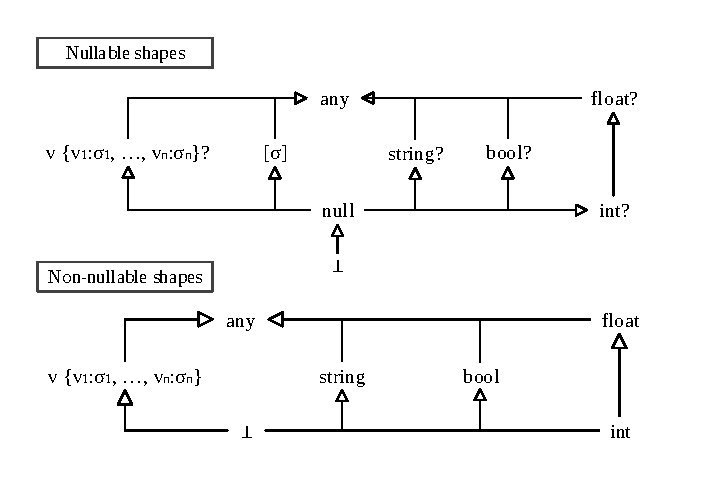
\includegraphics[scale=0.80,trim=5mm 5mm 5mm 5mm,clip]{images/hierarchy.pdf} % left bottom right top
\end{center}
\vspace{-0.5em}
\caption{Important aspects of the preferred shape relation}
\label{fig:subtyping-diagram}
\vspace{-0.5em}
\end{figure}

% -------------------------------------------------------------------------------------------------

\subsection{Inferred shapes}
\label{sec:inference-types}

We distinguish between \emph{non-nullable shapes} that always have a valid value (written as 
$\hat{\sigma}$) and \emph{nullable shapes} that encompass missing and \kvd{null} values 
(written as $\sigma$). We write $\nu$ for record names and record field names. 

\noindent
\begin{equation*}
\begin{array}{rcl}
 \hat{\sigma} &\narrow{=}& \nu \; \{ \nu_1 : \sigma_1, \ldots, \nu_n : \sigma_n, \rho_i  \} \\[0.1em]
                &\narrow{|}& \ident{float} \lsep \ident{int} \lsep \ident{bool} \lsep \ident{string} 
 \\[0.6em] 
       \sigma &\narrow{=}& ~\hat{\sigma}~ \lsep \kvd{nullable}\langl \hat{\sigma} \rangl \lsep [\sigma] \lsep \kvd{any} \lsep \kvd{null}  \lsep ~\bot~
\end{array}
\end{equation*}

\noindent
Non-nullable shapes include records (consisting of a name and fields with their shapes) and 
primitives. Names of records arising from XML are the names of the XML elements while
JSON records always use a single name $\bullet$.

We include two numerical primitives, \ident{int} for integers and \ident{float} for floating-point 
numbers. The two are related by the perference relation and we prefer \ident{int}.

Any non-nullable shape $\hat{\sigma}$ can be wrapped as $\kvd{nullable}\langl\hat{\sigma}\rangl$ to 
explicitly permit the \kvd{null} value. Type providers map \kvd{nullable} shapes to the F\# option
type. A collection $[\sigma]$ is also nullable and \kvd{null} values are treated as empty 
collections. The shape $\kvd{null}$ is inhabited by the $\kvd{null}$ value (using an overloaded 
notation) and $\bot$ is the bottom shape. The \kvd{any} shape is the top shape, but we revisit it 
later by adding labels for statically known alternative shapes (\S\ref{sec:inference-vars}) as 
discussed earlier (\S\ref{sec:providers-xml}).

In the rest of the paper, we assume that record fields can be freely reordered.

During inference we use row-variables $\rho_i$ in record shapes to represent the flexibility
arising from records in samples. For example, when a 
record {\small\ttfamily \{ x : 3 \}} occurs in a sample,
it may be combined through inference with other
samples such as {\small\ttfamily \{ x : 3, y : 4 \}} that contain more fields. The
overall shape inferred must account for the fact that any extra fields are optional,
giving an inferred shape {\small\ttfamily \{ x : int, y : option<int> \}}.
The process of solving $\rho_i$ variables is  discussed in \S\ref{sec:formal-inferval}. 


% -------------------------------------------------------------------------------------------------

\subsection{Preferred shape relation}
\label{sec:inference-subtyping}

Figure~\ref{fig:subtyping-diagram} provides an intuition about the preference between 
shapes. The upper part shows non-nullable shapes (with records and primitives) and the lower part 
shows nullable shapes with \kvd{null}, collections and nullable shapes. In the diagram, we 
abbreviate $\kvd{nullable}\langl\sigma\rangl$ as $\sigma?$ and we omit links between the two parts;
a shape $\hat{\sigma}$ is preferred over $\kvd{nullable}\langl\hat{\sigma}\rangl$.

\begin{definition}
For ground $\sigma_1$, $\sigma_2$ (i.e. without $\rho_i$ variables), we write $\sigma_1 \sqsupseteq \sigma_2$ to denote that $\sigma_2$ is preferred over $\sigma_1$. 
The shape preference relation is defined as a transitive reflexive closure of the following rules:

\noindent
\begin{align}
  \label{eq:sub-prim}\tag{P1}
  \ident{float}\,&\sqsupseteq\,\ident{int}&\\[-0.2em]
  \label{eq:sub-null}\tag{P2}
  \sigma &\sqsupseteq \kvd{null}  &(\textnormal{iff}~\sigma \neq \hat{\sigma})  \\[-0.2em]
  \label{eq:sub-opt}\tag{P3}
  \kvd{nullable}\langl\hat{\sigma}\rangl &\sqsupseteq \hat{\sigma}  &(\textnormal{for all}~\hat{\sigma})\\[-0.2em]
  \label{eq:sub-opt-cov}\tag{P4}
  \kvd{nullable}\langl\hat{\sigma_1}\rangl &\sqsupseteq 
    \kvd{nullable}\langl\hat{\sigma_2}\rangl  &(\textnormal{if}~\hat{\sigma_1} \sqsupseteq \hat{\sigma_2})\\[-0.2em]
  \label{eq:sub-col}\tag{P5}
  [\sigma_1] &\sqsupseteq [\sigma_2]  &(\textnormal{if}~\sigma_1 \sqsupseteq \sigma_2) \\[-0.2em]
  \label{eq:sub-bot}\tag{P6}
  \sigma &\sqsupseteq \bot  &(\textnormal{for all}~\sigma)\\[-0.2em]
  \label{eq:sub-var-top}\tag{P7}
  \kvd{any} &\sqsupseteq \sigma 
\end{align}
\vspace{-2em}

\noindent
\begin{align}
\label{eq:sub-record1}\tag{R1}
\begin{array}{l}
 \nu~\{ \nu_1\!:\!\sigma_1, .., \nu_n\!:\!\sigma_n \} \sqsupseteq \\
 \quad\nu~\{ \nu_1\!:\!\sigma_1', .., \nu_n\!:\!\sigma_n' \}
\end{array} \qquad ~~~~(\textnormal{if}~\sigma_i \sqsupseteq \sigma_i')
\end{align}

\vspace{-1.5em}

\begin{align}
\label{eq:sub-record2}\tag{R2}
\begin{array}{l}
 \nu~\{ \nu_1\!:\!\sigma_1, .., \nu_n\!:\!\sigma_n \} \sqsupseteq \\
 \quad\nu~\{ \nu_1\!:\!\sigma_1, .., .., \nu_m\!:\!\sigma_m \}
\end{array} \quad~~\, (\textnormal{when}~m \geq n)
\end{align}

\end{definition}

% --------------------------------------------------------------------------------------------------

\begin{figure*}[t]
\noindent
\begin{equation*}
\begin{array}{rclcl}
 \tytag &\narrow{=}& \ident{collection}  &\narrow{\lsep}& \ident{number} \\
        &\narrow{\lsep}& \ident{nullable} &\narrow{\lsep}& \ident{string}  \\
        &\narrow{\lsep}& \nu ~\lsep \ident{any} &\narrow{\lsep}& \ident{bool}
\end{array}
%
\quad\;\;\;
%
\begin{array}{rcl}
 \tytagof(\ident{string}) &\narrow{=}& \ident{string}\\
 \tytagof(\ident{bool}) &\narrow{=}& \ident{bool}\\
 \tytagof(\ident{int}) &\narrow{=}& \ident{number}\\
 \tytagof(\ident{float}) &\narrow{=}& \ident{number}\\
\end{array}
%
\;\;
%
\begin{array}{rcl}
 \tytagof(\kvd{any}\langl\sigma_1, \ldots, \sigma_n\rangl) &\narrow{=}& \ident{any}\\
 \tytagof(\nu\; \{ \nu_1 : \sigma_1, \; \ldots \; , \nu_n : \sigma_n \}) &\narrow{=}& \nu \\
 \tytagof(\kvd{nullable}\langl\hat{\sigma}\rangl) &\narrow{=}& \ident{nullable}\\
 \tytagof([\sigma]) &\narrow{=}& \ident{collection}\\
\end{array}
\end{equation*}

\vspace{-0.5em}
\begin{equation*}
\quad\qquad\qquad
\begin{array}{rcll}
 \addopt{\hat{\sigma}} &\narrow{=}& \kvd{nullable}\langl\hat{\sigma}\rangl &(\textnormal{non-nullable shapes})\\
 \addopt{\sigma} &\narrow{=}& \sigma &(\textnormal{otherwise})
\end{array}
\qquad\qquad
\begin{array}{rcll}
 \dropopt{\kvd{nullable}\langl\hat{\sigma}\rangl} &\narrow{=}& \hat{\sigma} &(\textnormal{nullable shape})\\
 \dropopt{\sigma} &\narrow{=}& \sigma &(\textnormal{otherwise})
\end{array}
\end{equation*}

\vspace{-0.5em}
\begin{equation*}
% option types
\inference[(nullable)\;]
  {\hat{\sigma_1} \tsep \sigma_2 \vdash \sigma}
  {\kvd{nullable}\langl\hat{\sigma_1}\rangl \tsep \sigma_2 \vdash \kvd{nullable}\langl\dropopt{\sigma}\rangl}
\qquad
\inference[(any)\;]
  { \tytagof(\sigma_1) \neq \tytagof(\sigma_2) & \tytagof(\sigma_1) \neq \ident{nullable} \neq \tytagof{\sigma_2}}
  { \sigma_1 \tsep \sigma_2 \vdash \kvd{any} }  
\end{equation*}
\vspace{-2em}

\begin{equation*}
\hspace{4em}
\inference[(record)\;]
  { \forall i\in\{ 1 .. n \}.(\sigma_i \tsep \sigma'_i \vdash \sigma''_i) }
  { \begin{array}{l}
    \nu \; \{ \nu_1 \!:\! \sigma_1,  \ldots \;, \nu_n \!:\! \sigma_n \} \tsep
    \nu \; \{ \nu'_1 \!:\! \sigma'_1, \; \ldots \;, \nu'_m \!:\! \sigma'_m \} \vdash
    \nu \; \{ \nu_1 \!:\! \sigma''_1, \; \ldots \; , \nu_k \!:\! \sigma''_n \}
    \end{array} }
\end{equation*}
\vspace{-2em}

% all rules are symmetric and reflexive
\begin{equation*}
\hspace{2em}
\inference[(list)\;]
  {\sigma_1 \tsep \sigma_2 \vdash \sigma}
  {[\sigma_1] \tsep [\sigma_2] \vdash [\sigma]}
\quad
\inference[(sym)\;]
  {\sigma_1 \tsep \sigma_2 \vdash \sigma}
  {\sigma_2 \tsep \sigma_1 \vdash \sigma}
%
\quad
\begin{array}{l}
 \textnormal{\footnotesize{(refl)}}\;\; \sigma \tsep \sigma \vdash \sigma\\[0.6em]
 % bottom type
 \textnormal{\footnotesize{(bot)}}\;\; \bot \tsep \sigma \vdash \sigma
\end{array}
%
\quad
% null and primitives
\begin{array}{l}
 \textnormal{\footnotesize{(null)}}\;\; \sigma \tsep \kvd{null} \vdash \addopt{\sigma} \quad (\sigma \neq \bot)\\[0.6em]
 \textnormal{\footnotesize{(prim)}}\;\; \kvd{int} \tsep \kvd{float} \vdash \kvd{float}
\end{array}
\end{equation*}

\caption{The common preferred shape relation}
\label{fig:subtyping-cst}
\end{figure*}

% --------------------------------------------------------------------------------------------------


\noindent
Here is a summary of the key aspects of the definition:
\begin{itemize}
\item Numeric shape with smaller range is preferred (\ref{eq:sub-prim}) and we choose 32-bit 
\ident{int} over \ident{float} when possible.

\item The \kvd{null} shape is preferred over all nullable shapes (\ref{eq:sub-null}), i.e. 
  all shapes excluding non-nullable shapes $\hat{\sigma}$. Any non-nullable shape is preferred
  over its nullable version (\ref{eq:sub-opt}); nullable shapes and collections are 
  covariant (\ref{eq:sub-opt-cov}, \ref{eq:sub-col}).

\item There is a bottom shape (\ref{eq:sub-bot}) and \kvd{any} behaves as the top shape, because
  any shape $\sigma$ is preferred over \kvd{any} (\ref{eq:sub-var-top}). 

\item The record shapes are covariant (\ref{eq:sub-record1}) and preferred record can have 
  additional fields (\ref{eq:sub-record2}). 
\end{itemize}

\noindent

% -------------------------------------------------------------------------------------------------

\subsection{Common preferred shape relation}
\label{sec:inference-commonsuper}

Given two ground shapes, the \emph{common preferred shape} relation finds a least upper bound
(Lemma~\ref{thm:lub}). It prefers records, which is important for usability as discussed
earlier.

\begin{definition}
A \emph{common preferred shape} of two ground shapes $\sigma_1$ and $\sigma_2$ is a shape $\sigma$, written 
$\sigma_1 \tsep \sigma_2 \vdash \sigma$, by the rules in 
Figure~\ref{fig:subtyping-cst}.
\end{definition}

\noindent
We define shape \emph{tags} to identify shapes that have a common preferred shape which is not the
top shape. When finding a common shape of two records (\emph{record}), the shape of fields becomes the common preferred shape of their 
respective shapes. If the field labels of two record types do not match,
we can assume a common assignment of fields has been determined
through shape inference (\S\ref{sec:formal-inferval}).

We can find a common shape of two different numbers (\emph{prim}); for two collections,
we combine their elements (\emph{list}). When one shape is nullable (\emph{nullable}), we find
the common non-nullable shape and wrap it in \kvd{nullable}; if one of the shapes is \kvd{null}, 
we make the other one nullable (\emph{null}). Finally, if the two shapes do not have matching tags 
(and they are not nullable), we have to infer the \kvd{any} shape as there is no better alternative. 
The remaining rules for reflexivity, symmetry and the bottom shape are standard.

\paragraph{Properties.}
A set of ground shapes has a \emph{unique} least upper bound by the preferred shape ordering.
For ground shapes, the common preferred shape relation defines a function (Lemma~\ref{thm:func}) that finds 
the least upper bound (Lemma~\ref{thm:lub}). 

\begin{lemma}[Preferred shape function]
\label{thm:func}
For all ground $\sigma_1$ and $\sigma_2$ there exists exactly one $\sigma$ such that 
$\sigma_1 \tsep \sigma_2 \vdash \sigma$. 
\end{lemma}
\begin{proof}
The pre-conditions of rules in Figure~\ref{fig:subtyping-cst} are disjoint, with the exception 
of (\emph{sym}) and (\emph{refl}), but applying those does not affect the result. Reflexivity is
preserved recursively and all rules, symmetry does not enable different derivations, even for
non-symmetric (\emph{nullable}) and (\emph{prim}).
\end{proof}

\begin{lemma}[Least upper bound]
\label{thm:lub}
For ground $\sigma_1$ and $\sigma_2$, if $\sigma_1 \triangledown \sigma_2 \vdash \sigma$ then $\sigma$ is a least upper bound by $\sqsupseteq$.
\end{lemma}
\begin{proof}
By induction over $\vdash$. The algorithm only infers the top shape \kvd{any} when for non-nullable
shapes of distinct tags and so no better preferred shape exists.
\end{proof}

\subsection{Inferring shapes from samples}
\label{sec:formal-inferval}

We now specify how we obtain the shape from data. We represent JSON, XML and CSV documents using
the same first-order \emph{data} value (\S\ref{sec:impl-parsing}):
%
\begin{equation*}
\begin{array}{lcl}
 d &\narrow{=}& i \lsep f \lsep s \lsep \kvd{true} \lsep \kvd{false} \lsep \kvd{null} \\[0.1em]
   &\narrow{|}& [d_1; \ldots; d_n] \lsep \nu~\{ \nu_1 \mapsto d_1, \ldots, \nu_n \mapsto d_n \}
\end{array}
\end{equation*}
%
The first few cases of represent primitive values ($i$ for integers, $f$ for floating
point numbers and $s$ for strings) and the \kvd{null} value. A collection is written as a 
list of values in square brackets. A record starts with a name $\nu$, followed by a 
sequence of field assignments $\nu_i \mapsto d_i$.

Figure~\ref{fig:shape-inference} defines a mapping $\semalt{d_1,\ldots,d_n}$ which turns a collection of sample 
data $d_1, \ldots, d_n$ into a shape $\sigma$. Before applying $S$, we assume each record in each $d_i$ is marked with a fresh row inference
variable $\rho_i$.  
We then choose a ground, minimal substitution $\theta$ for row variables.
Because $\rho_i$ variables represent potentially missing fields,
the $\addopt{-}$ operator from Figure~\ref{fig:subtyping-cst} is applied to all types
in the vector. 
This must be sufficient to equate the record field labels and satisfy the side conditions in rule (record) when multiple record samples are merged.
In practice, $\theta$ is found via row variable unification, we omit the details here.
No $\rho_i$ variables remain after inference as the substitution chosen is ground.



\begin{figure}
\noindent
\begin{equation*}
\begin{array}{rclcrclcrcl}
 \semalt{i} &\narrow{=}& \ident{int} && \semalt{\kvd{null}}  &\narrow{=}& \kvd{null} && \semalt{\kvd{true}} &\narrow{=}& \ident{bool}\\
 \semalt{f} &\narrow{=}& \ident{float} && \semalt{s} &\narrow{=}& \ident{string} && \semalt{\kvd{false}}  &\narrow{=}& \ident{bool}\\
\end{array}
\end{equation*}
\noindent
\vspace{-0.5em}
\begin{equation*}
\begin{array}{l}
 \semalt{[d_1; \ldots; d_n]} = [\semalt{d_1, \ldots, d_n}]
 \\[0.5em]
 \semalt{\nu~\{ \nu_1 \mapsto d_1, \ldots, \nu_n \mapsto d_n \}_{\rho_i}} =\\[0.1em]
 \qquad\nu~\{ \nu_1:\semalt{d_1}, \ldots, \nu_n :\semalt{d_n}, \addopt{\theta(\rho_i)} \}
 \\[0.5em]
 \semalt{d_1, \ldots, d_n} = \sigma_n \quad\textnormal{where}\\[0.1em]
 \qquad\sigma_0 = \bot,~ \forall i\in \{ 1.. n \}.~ \sigma_{i-1} \triangledown \semalt{d_i} \vdash \sigma_i \\[0.1em]
 \textnormal{Choose minimal}\ \theta\ \textnormal{by ordering}\ \sqsupseteq\ \textnormal{lifted over substitutions} \\[0.1em]
\end{array}
\end{equation*}
\caption{Shape inference}
\label{fig:shape-inference}
\end{figure}

%
Primitive  values are mapped to their corresponding shapes. 
When infering a shape from multiple samples, we use the common preferred shape relation to find a 
common shape for all values (starting with $\bot$). This operation is used at the top-level 
(when calling a type provider with multiple samples) and also when inferring the shape of collection
elements.




% --------------------------------------------------------------------------------------------------

\begin{figure*}
  \noindent
  \begin{equation*}
  \textnormal{\footnotesize{(top-1)}}\;\;
  \inference
    {\exists i . \tytagof(\sigma_i) = \tytagof(\dropopt{\sigma}) & \sigma \tsep \sigma_i \vdash \sigma_i' & \tytagof(\sigma)\neq\ident{any}}
    {\sigma \tsep \kvd{any}\langl\sigma_1, \ldots, \sigma_n\rangl \vdash 
      \kvd{any}\langl\sigma_1, \ldots, \dropopt{\sigma_i'}, \ldots, \sigma_n\rangl}
  \;\;
  \inference
    {\nexists i . \tytagof(\sigma_i) = \tytagof(\dropopt{\sigma}) & \tytagof(\sigma)\neq\ident{any}}
    {\sigma \tsep \kvd{any}\langl\sigma_1, \ldots, \sigma_n\rangl \vdash 
      \kvd{any}\langl\sigma_1, \ldots, \sigma_n, \dropopt{\sigma}\rangl}
  \end{equation*}
  \vspace{-2em}

  % two union types
  \begin{equation*}
  \begin{array}{l}
  \inference[(top-2)\;]
    { (\tytagof(\sigma_i) = \tytagof(\sigma'_j)) \Leftrightarrow (i = j) \wedge (i \leq k)\\
        \forall i\in\{ 1 .. k \}.(\sigma_i \tsep \sigma'_i \vdash \sigma''_i) }
    { \begin{array}{l}
      \kvd{any}\langl \sigma_1, \ldots, \sigma_k,  \ldots, \sigma_n\rangl \tsep 
      \kvd{any}\langl \sigma'_1, \ldots, \sigma'_k, \ldots, \sigma'_m\rangl \vdash\\
      \kvd{any}\langl \sigma''_1, \ldots, \sigma''_k, \sigma_{k+1}, \ldots, \sigma_{n}, \sigma'_{k+1}, \ldots, \sigma'_{m}\rangl
      \end{array} }
  \end{array}    
  \begin{array}{l}
  \inference[(top-3)\;]
    {(\forall i\in\{1,2\}) & \tytagof(\sigma_1) \neq \tytagof(\sigma_2) \\ 
     \tytagof(\sigma_i) \neq \ident{any} & \nexists\sigma_i' . (\sigma_i = \kvd{option}\langl\sigma_i'\rangl)  }
    {\sigma_1 \tsep \sigma_2 \vdash \kvd{any}\langle\dropopt{\sigma_1}, \dropopt{\sigma_2}\rangle}
  \end{array}  
  \end{equation*}
  \caption{Extending the common preferred shape relation for labelled top shapes}
  \label{fig:subtyping-cst-var}
\end{figure*}

% --------------------------------------------------------------------------------------------------

\subsection{Adding labelled top shapes}
\label{sec:inference-vars}

Next, we indicate how the core model (sufficient for the relativized safety) 
can be extended with \emph{labelled top shapes} discussed earlier.

When analyzing the structure of shapes, it suffices to consider a single top shape \kvd{any}.
However, the type providers need more information to provide typed access to the possible 
alternative shapes of data, such as XML nodes. To support track the possible shapes, we label 
the \kvd{any} shape:
%
\begin{equation*}
\sigma = \ldots \lsep \kvd{any}\langl \sigma_1, \ldots, \sigma_n\rangl
\end{equation*}
%
The shapes $\sigma_1, \ldots, \sigma_n$ represent statically known shapes that appear in the
sample and that we expose in the provided type. As discussed earlier (\S\ref{sec:providers-xml})
this is important when reading external \emph{open world} data. The labels do not affect the 
preferred shape relation and $\kvd{any}\langl \sigma_1, \ldots, \sigma_n\rangl$ should still be
seen as the top shape, regardless of the labels.

The common preferred shape relation is extended to find a labelled top shape that best represents 
the sample. We limit the number of labels and avoid nesting by grouping shapes by the shape tag 
introduced earlier (Figure~\ref{fig:subtyping-cst}).
For example, rather than inferring $\kvd{any}\langl\ident{int}, \kvd{any}\langl\ident{bool}, \ident{float}\rangl\rangl$, 
our algorithm finds the common preferred shape of $\ident{int}$ and $\ident{float}$ and produces 
$\kvd{any}\langl\ident{float},\ident{bool}\rangl$. 

The three rules in Figure~\ref{fig:subtyping-cst-var} replace the earlier (\emph{top}). When 
combining a top with another shape (\emph{top-1}), the labelled top shape may or may not already 
contain a case with the tag of the other shape. If it does, the two shapes are combined, otherwise 
a new case is added. When combining two top shapes (\emph{top-2}), we group the labels that have 
shared tags. Finally, (\emph{top-3}) covers the case when we are combining two distinct non-top 
shapes. As top shapes implicitly permit \kvd{null} values, we use an auxiliary function $\dropopt{-}$ 
to make nullable shapes non-nullable (when possible) to simplify the label.

\paragraph{Properties.}
The revised algorithm still finds a shape which is the least upper bound. This means that 
labelled top shape is only inferred when there is no other alternative.

Stating properties of the labels requires refinements to the \emph{preferred shape} relation.
We leave the details to future work, but we
note that the algorithm infers the best labels in the sense that there are labels that enable 
typed access to every possible value in the sample, but not more. The same is the case for nullable
fields of records.


% ==================================================================================================
% 
%    #######
%    #        ####  #####  #    #   ##   #      # ######   ##   ##### #  ####  #    #
%    #       #    # #    # ##  ##  #  #  #      #     #   #  #    #   # #    # ##   #
%    #####   #    # #    # # ## # #    # #      #    #   #    #   #   # #    # # #  #
%    #       #    # #####  #    # ###### #      #   #    ######   #   # #    # #  # #
%    #       #    # #   #  #    # #    # #      #  #     #    #   #   # #    # #   ##
%    #        ####  #    # #    # #    # ###### # ###### #    #   #   #  ####  #    #
%
% ==================================================================================================

\section{Formalising type providers}
\label{sec:formal}

This section presents the formal model of type providers for structured data. 
To represent the programming language that hosts the type provider and the
provided declarations, we introduce the Foo calculus,
a subset of F\# using object-property notation with
added operations for working with weakly typed structured data along the lines of the F\# Data runtime. Finally, we describe how 
type providers turn inferred shapes into Foo classes (\S\ref{sec:formal-tp}).

Type providers for structured data map the ``dirty'' world of weakly typed 
semi-structured data into a ``nice'' world of strong types. To model this, the Foo calculus
does not have \kvd{null} values and data values $d$ are never directly exposed.  
Furthermore Foo is simply typed: despite using class types and object notation 
for notational convenience, it has no subtyping.

% -------------------------------------------------------------------------------------------------

\begin{figure*}
\noindent
\begin{equation*}
\hspace{1.1em}
\begin{array}{l}
\ident{hasShape}(\nu~ \{ \nu_1 \!:\! \sigma_1, \ldots, \nu_n \!:\! \sigma_n \}, \nu'~\{ \nu'_1\mapsto d_1, \ldots, \nu'_m\mapsto d_m \}) \reduce (\nu = \nu') ~\wedge \\
  \quad (~ ((\nu_1 = \nu'_1) \wedge \ident{hasShape}(\sigma_1, d_1)) \vee\ldots\vee ((\nu_1 = \nu'_m) \wedge \ident{hasShape}(\sigma_1, d_m)) \vee \ldots \vee\\
  \quad ~\; ((\nu_n = \nu'_1) \wedge \ident{hasShape}(\sigma_n, d_1)) \vee\ldots\vee ((\nu_n = \nu'_m) \wedge \ident{hasShape}(\sigma_n, d_m))~)
\\[0.5em]
\ident{hasShape}([\sigma], [d_1; \ldots; d_n]) \reduce \ident{hasShape}(\sigma, d_1)\wedge\ldots\wedge\ident{hasShape}(\sigma, d_n) \\
\ident{hasShape}([\sigma], \kvd{null}) \reduce \kvd{true} 
\end{array}  
\quad
\begin{array}{l}
\ident{convFloat}(\ident{float}, i) \reduce f~(f=i) \\
\ident{convFloat}(\ident{float}, f) \reduce f \\[0.75em]
\ident{convNull}(\kvd{null}, e) \reduce \ident{None} \\
\ident{convNull}(d, e) \reduce \ident{Some}(e~d) 
\end{array}
\end{equation*}
%
\vspace{-0.75em}
%
\begin{equation*}
\begin{array}{l}
\ident{hasShape}(\ident{string}, s) \reduce \kvd{true} \\
\ident{hasShape}(\ident{int}, i) \reduce \kvd{true}\\
\ident{hasShape}(\ident{bool}, d) \reduce \kvd{true} \quad(\textnormal{when}~d\in{\kvd{true},\kvd{false}} )\\
\ident{hasShape}(\ident{float}, d) \reduce \kvd{true} \quad(\textnormal{when}~d=i ~\textnormal{or}~ d=f) \\
\ident{hasShape}(\_, \_) \reduce \kvd{false} \\
\end{array}
\;\;
\begin{array}{l}
\ident{convPrim}(\sigma, d) \reduce d\quad(\sigma,d\in\{ (\ident{int},i),(\ident{string},s),(\ident{bool}, b) \})
\\[0.25em]
\ident{convField}(\nu,\nu_i, \nu~\{\ldots, \nu_i=d_i, \ldots\}, e) \reduce e~d_i\\
\ident{convField}(\nu,\nu', \nu~\{\ldots, \nu_i=d_i, \ldots\}, e) \reduce e~\kvd{null}\quad(\nexists i.\nu_i=\nu' )
\\[0.25em]
\ident{convElements}([d_1; \ldots; d_n], e) \reduce e~d_1 :: \ldots :: e~d_n :: \kvd{nil}  \\  
\ident{convElements}(\kvd{null}) \reduce \kvd{nil}
\end{array}
\end{equation*}

\caption{Reduction rules for conversion functions}
\label{fig:op-conversions}
\vspace{-0.5em}
\end{figure*}

% --------------------------------------------------------------------------------------------------

\subsection{The Foo calculus}
\label{sec:formal-ff}

The syntax of the calculus is shown in Figure~\ref{fig:foo-syntax}. We only need classes with 
parameter-less members and without inheritance. A class has a single implicit constructor and the 
declaration closes over constructor parameters. 

The type \ident{Data} is the type of structural data $d$. A class definition $L$ consists of 
a constructor and zero or more members. Values $v$ include previously defined data $d$; expressions
$e$ include class construction, member access and the usual functional constructs (functions,
lists, options) and conditionals. The $op$ constructs are discussed next.

% -------------------------------------------------------------------------------------------------

\paragraph{Dynamic data operations.}

The Foo programs can only work with \ident{Data} values using certain primitive operations. Those are modelled
by the $op$ primitives. In F\# Data, those are internal and users never access them directly.

% -------------------------------------------------------------------------------------------------

\begin{figure}[!h]
\noindent
\begin{equation*}
\begin{array}{rcl}
 \tau &\narrow{=}& \ident{int} \lsep \ident{float} \lsep \ident{bool} \lsep \ident{string} \lsep C \lsep \ident{Data} \\[0.0em]
      &\narrow{|}& \tau_1 \rightarrow \tau_2 \lsep \ident{list}\langl\tau\rangl \lsep \ident{option}\langl\tau\rangl 
\\[0.6em]
 L &\narrow{=}& \kvd{type}~C(\overline{x:\tau}) = \overline{M} \\[0.0em]
 M &\narrow{=}& \kvd{member}~N:\tau= e
\\[0.6em]
 v &\narrow{=}& d \lsep \ident{None} \lsep \ident{Some}(v) \lsep \kvd{new}~C(\overline{v}) \lsep v_1::v_2 \\[0.0em]
 e &\narrow{=}& d \lsep op \lsep e_1~e_2 \lsep \lambda x.e \lsep e.N \lsep \kvd{new}~C(\overline{e}) \\
   &\narrow{|}& \ident{None} \lsep\kvd{match}~e~\kvd{with}~\ident{Some}(x) \rightarrow e_1 \,|\, \ident{None} \rightarrow e_2 \\
   &\narrow{|}& \ident{Some}(e) \lsep e_1 = e_2 \lsep {\kvd{if}~e_1~\kvd{then}~e_2~\kvd{else}~e_3} \lsep \kvd{nil} \\
   &\narrow{|}& e_1 :: e_2 \lsep \kvd{match}~e~\kvd{with}~x_1::x_2 \rightarrow e_1 \,|\, \kvd{nil} \rightarrow e_2 
\\[0.6em]
op &\narrow{=}& \ident{convFloat}(\sigma, e) \lsep \ident{convPrim}(\sigma, e) \\
   &\narrow{|}& \ident{convField}(\nu_1, \nu_2, e, e) \lsep \ident{convNull}(e_1, e_2) \\
   &\narrow{|}& \ident{convElements}(e_1, e_2) \,\lsep \ident{hasShape}(\sigma, e) 
\end{array}
\end{equation*}

\caption{The syntax of the Foo calculus}
\label{fig:foo-syntax}
\vspace{-0.5em}
\end{figure}

% -------------------------------------------------------------------------------------------------

The behaviour of the dynamic data operations is defined by the reduction rules in 
Figure~\ref{fig:op-conversions}. The operations can convert data values into values of 
less preferred shape. For example, \ident{convFloat} turns an integer \num{1} into 
a floating-point \num{1.0} and \ident{convElements} turns \kvd{null} value into an empty list.

All of the dynamic data operations take a data value $d$ and produce a Foo value. We do not 
make the conversion explicit for primitive values (\ident{convPrim}) and assume that primitive
values are shared, but we convert all other values. For example \ident{convElements} turns a 
data collection $[d_1, \ldots, d_n]$ into a Foo list $v_1 :: .. :: v_n :: \kvd{nil}$.

The data operations for collections, record fields and nullable values all take a function
as the last argument and invoke it to convert the obtained data. For example, \ident{convField} 
accesses a record field -- it ensures that the actual record name matches the expected name and 
passes the field value (or \kvd{null} data value) to the provided function.

Finally, we also define a runtime shape test \ident{hasShape}.
The most complex case is handling of records where we check that for each field $\nu_1, \ldots, \nu_n$ 
in the record, the actual record value has a field of the same name with a matching shape. The last 
line defines a ``catch all'' pattern, which returns \kvd{false} for all remaining cases. 
We treat $e_1 \vee e_2$ and $e_1 \wedge e_2$ as syntactic sugar for \kvd{if}-\kvd{then}-\kvd{else} so
the rule is expressed using just Foo expressions.

% -------------------------------------------------------------------------------------------------

\paragraph{Reduction.}
The reduction relation is of the form $L, e \reduce e'$. We omit class declarations 
$L$ where implied by context and write $e \reduce^{*} e'$ for
the reflexive, transitive closure of $\reduce$. 

Figure~\ref{fig:ff-reduction} shows the reduction rules. The (\emph{ctx}) rule models the eager
evaluation of F\# and performs a reduction inside a sub-expression specified by an evaluation 
context $E$:
%
\begin{equation*}
\begin{array}{rcl}
 E &\narrow{=}& v::E \lsep v~E \lsep E.N \lsep \kvd{new}~C(\overline{v}, E, \overline{e})\\[0.1em]
   &\narrow{|}&  \kvd{if}~E~\kvd{then}~e_1~\kvd{else}~e_2  \lsep E = e \lsep v = E \\[0.1em]
   &\narrow{|}& \ident{Some}(E) \lsep op(\overline{v}, E, \overline{e})\\[0.1em]
   &\narrow{|}& \kvd{match}~E~\kvd{with}~\ident{Some}(x) \rightarrow e_1 \,|\, \ident{None} \rightarrow e_2 \\[0.1em]
   &\narrow{|}& \kvd{match}~E~\kvd{with}~x_1 :: x_2 \rightarrow e_1 \,|\, \kvd{nil} \rightarrow e_2
\end{array} 
\end{equation*}

\noindent
The evaluation proceeds from left to right as denoted by $\overline{v}, E, \overline{e}$ in 
constructor and dynamic data operation arguments or $v::E$ in list initialization.

We write $e[\overline{x} \leftarrow \overline{v}]$ for the result of replacing variables $\overline{x}$ by
values $\overline{v}$ in an expression. The (\emph{member}) rule reduces a member access using a class 
definition in the assumption to obtain the body of a member. The remaining six rules
give standard reductions.

% -------------------------------------------------------------------------------------------------

\paragraph{Type checking.} 
Well-typed Foo programs reduce to a value in a finite number of steps or get stuck due to an
error condition. The stuck states can only be due to the dynamic data operations (e.g.
$\ident{convFloat}(\ident{float},\kvd{null})$). The relativized type safety (Theorem~\ref{thm:safety})
characterizes the additional conditions on input data under which Foo programs do not ``go wrong''.

Typing rules in Figure~\ref{fig:ff-typecheck} are written using a judgement
$L; \Gamma \vdash e : \tau$ where the context also contains a set of class declarations $L$.
The fragment demonstrates the differences and similarities with Featherweight Java \cite{fwjava}:
%
\begin{itemize}
\item[--] All data values $d$ have the type \ident{Data}, but primitive data values (Booleans, 
  strings, integers and floats) can be implicitly converted to Foo values and so they also have a 
  primitive type as illustrated by the rule for $i$ and $f$.
\item[--] For non-primitive data values (including \kvd{null}, data collections and records),
  \ident{Data} is the only type.
\item[--] Operations $op$ (omitted) have a family of types (Foo does not have polymorphic types),
  accepting \ident{Data} as one of the arguments and producing a non-\ident{Data} Foo type.
\item[--] Rules for checking class construction and member access are similar to corresponding
  rules of Featherweight Java.  
\end{itemize}
%
An important part of Featherweight Java that is omitted here is the checking of type declarations
(ensuring the members are well-typed). We consider only classes generated by our type providers 
and those are well-typed by construction.

% -------------------------------------------------------------------------------------------------

\begin{figure}
\noindent
\begin{equation*}
\begin{array}{rl}
 \textnormal{\footnotesize{(member)}}&
 \hspace{-0.6em}
 \inference
 { \kvd{type}~C(\overline{x:\tau})= \kvd{member}~N_i : \tau_i = e_i \ldots \in L }
 { L, (\kvd{new}~C(\overline{v})).N_i \reduce e_i[\overline{x} \leftarrow \overline{v}] }\\
 \\[-0.2em]
 \textnormal{\footnotesize{(match1)}}&
 \hspace{-1em}
 \begin{array}{l}
  \kvd{match}~\ident{None}~\kvd{with} \\
  \ident{Some}(x) \rightarrow e_1 \,|\, \ident{None} \rightarrow e_2
 \end{array} \hspace{-0.5em} ~\reduce~ e_2 \\
 \\[-0.2em]
 \textnormal{\footnotesize{(match2)}}&
 \hspace{-1em}
 \begin{array}{l}
    \kvd{match}~\ident{Some}(v)~\kvd{with} \\
    \ident{Some}(x) \rightarrow e_1 \,|\, \ident{None} \rightarrow e_2
 \end{array} \hspace{-0.5em} ~\reduce~ e_1[x\leftarrow v]\\
 \\[-0.2em]
 \textnormal{\footnotesize{(match3)}}&
 \hspace{-1em}
 \begin{array}{l}
  \kvd{match}~\kvd{nil}~\kvd{with} \\[0em]
  x_1::x_2 \rightarrow e_1 \,|\, \kvd{nil} \rightarrow e_2
 \end{array} \hspace{-0.5em} ~\reduce~ e_2\\
 \\[-0.2em]
 \textnormal{\footnotesize{(match4)}}&
 \hspace{-1em}
 \begin{array}{l}
  \kvd{match}~v_1::v_2~\kvd{with} \\[0em]
  x_1::x_2 \rightarrow e_1 \,|\, \kvd{nil} \rightarrow e_2
 \end{array} \hspace{-0.5em} ~\reduce~ e_1[\overline{x}\leftarrow\overline{v}] \\
 \\[-0.2em]
 \textnormal{\footnotesize{(cond1)}}&
 \hspace{-0.4em}
 \kvd{if}~\kvd{true}~\kvd{then}~e_1~\kvd{else}~e_2 ~\reduce~ e_1 \\
 \\[-0.2em]
 \textnormal{\footnotesize{(cond2)}}&
 \hspace{-0.4em}
 \kvd{if}~\kvd{false}~\kvd{then}~e_1~\kvd{else}~e_2 ~\reduce~ e_2 \\
 \\[-0.3em]
 \textnormal{\footnotesize{(eq1)}}&
 v=v\reduce\kvd{true} \qquad \textnormal{\footnotesize{(eq2)}}~~v=v'\reduce\kvd{false}\\
 \\[-0.3em]
 \textnormal{\footnotesize{(fun)}}&
 \hspace{-0.4em}
 (\lambda x.e)~v ~\reduce~ e[x\leftarrow v] \\
 \\[-0.3em]
 \textnormal{\footnotesize{(ctx)}}&
 \hspace{-0.4em}
  E[e] \reduce E[e'] \qquad\qquad(\textnormal{when}~e \reduce e')\\
\end{array}
\end{equation*}

\caption{Foo -- Remaining reduction rules}
\label{fig:ff-reduction}
\end{figure}

% -------------------------------------------------------------------------------------------------

\subsection{Type providers}
\label{sec:formal-tp}

So far, we defined the type inference algorithm which produces a shape $\sigma$ from one 
or more sample documents (\S\ref{sec:inference}) and we defined a simplified model of evaluation
of F\# (\S\ref{sec:formal-ff}) and F\# Data runtime (\S\ref{sec:formal-tp}). In this section, we 
define how the type providers work, linking the two parts.

All F\# Data type providers take (one or more) sample documents, infer a common preferred shape $\sigma$
and then use it to generate F\# types that are exposed to the programmer.\footnote{The actual 
implementation provides \emph{lazy erased types} as described in \cite{fsharp-typeprov}. Here, we treat 
the code as actually generated. This is an acceptable simplification, because F\# Data type providers 
do not rely on laziness or erasure of type provision.}

\paragraph{Type provider mapping.}
A type provider produces an F\# type $\tau$ together with a Foo expression and a collection of 
class definitions. We express it using the following mapping:
%
\begin{equation*}
\sem{-} : \sigma \rightarrow (\tau \times e \times L) \qquad (\textnormal{where}~L,\emptyset \vdash e:\ident{Data}\rightarrow\tau)
\end{equation*}
%
The mapping $\sem{\sigma}$ takes an inferred shape $\sigma$. It returns an F\# type $\tau$ and
a function that turns the input data (value of type \ident{Data}) into a Foo value of type $\tau$. 
The type provider also generates class definitions that may be used by $e$. 

Figure~\ref{fig:tp-generation} defines $\sem{-}$. Primitive types are handled by a single rule that
inserts an appropriate conversion function; \ident{convPrim} just checks that the shape matches
and \ident{convFloat} converts numbers to a floating-point.

For records, we generate a class $C$ that takes a data value as constructor parameter. For each 
record field, we generate a member with the same name as the field. The body of the member calls 
\ident{convField} with a function obtained from $\sem{\sigma_i}$. This function turns the field 
value (data of shape $\sigma_i$) into a Foo value of type $\tau_i$. The returned expression creates a new instance of 
$C$ and the mapping returns the class $C$ together with all recursively generated classes. Note that 
the class name $C$ is not directly accessed by the user and so we can use an arbitrary name, although the 
actual implementation in F\# Data attempts to infer a reasonable name.\footnote{For example, in 
\ident{\{\str{person}:\{\str{name}:\str{Tomas}\}\}}, the nested record will be named \ident{Person}
based on the name of the parent record field.}

A collection shape becomes a Foo $\ident{list}\langl\tau\rangl$. The returned expression calls \ident{convElements}
(which returns the empty list for data value \kvd{null}). The last parameter is the recursively obtained
conversion function for the shape of elements $\sigma$. The handling of the nullable shape is similar,
but uses \ident{convNull}.

As discussed earlier, labelled top shapes are also generated as Foo classes with properties. Given 
$\kvd{any}\langl\sigma_1, \ldots, \sigma_n\rangl$, we get corresponding F\# types $\tau_i$ and generate 
$n$ members of type $\ident{option}\langl \tau_i\rangl$. When the member is accessed, we need to perform
a runtime shape test using \ident{hasShape} to ensure that the value has the right shape (similarly to runtime 
type conversions from the top type in languages like Java). If the shape matches, a \ident{Some} value is 
returned. The shape inference algorithm also guarantees that there is only one case for each shape tag 
(\S\ref{sec:inference-commonsuper}) and so we can use the tag for the name of the generated member.

% -------------------------------------------------------------------------------------------------

\begin{figure}
\noindent  
\begin{equation*}
\inference
  {~}
  {L; \Gamma \vdash d : \ident{Data}}
~~
\inference
  {~}
  {L; \Gamma \vdash i : \ident{int}}
~~
\inference
  {~}
  {L; \Gamma \vdash f : \ident{float}}
\end{equation*}
\vspace{0.25em}
\begin{equation*}
\inference
  {L; \Gamma, x : \tau_1 \vdash e : \tau_2}
  {L; \Gamma \vdash \lambda x.e : \tau_2}
\quad
\inference
  {L; \Gamma \vdash e_2 : \tau_1 \\
   L; \Gamma \vdash e_1 : \tau_1 \rightarrow \tau_2}
  {L; \Gamma \vdash e_1~e_2 : \tau_2}
\end{equation*}
\vspace{0.5em}
\begin{equation*}
\inference
  {L; \Gamma \vdash e : C \\ \kvd{type}~C(\overline{x:\tau}) = ..\;\kvd{member}~N_i : \tau_i = e_i\;.. \in L}
  {L; \Gamma \vdash e.N_i:\tau_i}
\end{equation*}
\vspace{0.25em}
\begin{equation*}
\inference
  {L; \Gamma \vdash e_i : \tau_i & \kvd{type}~C(x_1:\tau_1, \ldots, x_n:\tau_n) = \ldots \in L}
  {L; \Gamma \vdash \kvd{new}~C(e_1, \ldots, e_n):C}
\end{equation*}

\caption{Foo -- Fragment of type checking}
\label{fig:ff-typecheck}
\end{figure}

% -------------------------------------------------------------------------------------------------

\begin{figure*}
\begin{multicols}{2}

% Primitives 
\noindent
\begin{equation*}
\begin{array}{l} 
 \sem{\sigma_p} = \tau_p,\lambda x\rightarrow op(\sigma_p, x),\emptyset\quad\textnormal{where} \\[0.6em] 
 \quad\sigma_p, \tau_p, op\in  \{~ (\ident{bool}, \ident{bool}, \ident{convPrim})\\
 \hspace{2.9em} (\ident{int}, \ident{int}, \ident{convPrim}), (\ident{float},\ident{float},\ident{convFloat}),\\
 \hspace{2.9em} (\ident{string},\ident{string},\ident{convPrim}) ~\}
\end{array} 
\end{equation*}
\vspace{-2em}

% Records
\begin{equation*}
\begin{array}{l}
 \sem{\,\nu~ \{ \nu_1 : \sigma_1, \ldots, \nu_n : \sigma_n \}\,} = \\[0.1em]
 \quad C, \lambda x\rightarrow \kvd{new}~C(x), L_1\cup\ldots\cup L_n\cup\{ L \}\quad\textnormal{where}\\[0.6em]
 \qquad \;\;C~\textnormal{is a fresh class name} \\
 \qquad \;\,\,L = \kvd{type}~C(x_1\!:\!\ident{Data})=M_1 \ldots M_n \\
 \qquad M_i = \kvd{member}~\nu_i:\tau_i=\ident{convField}(\nu, \nu_i, x_1, e_i),\\
 \qquad \tau_i, e_i, L_i = \sem{\sigma_i} 
\end{array}
\end{equation*}
\vspace{-2em}

% Collections
\begin{equation*}
\begin{array}{l}
 \sem{\,[\sigma]\,} = \ident{list}\langl\tau\rangl, \lambda x \rightarrow \ident{convElements}(x, e'), L \;\;\textnormal{where}\\[0.4em]
 \qquad \tau, e', L = \sem{\hat{\sigma}}
\end{array}
\end{equation*}

% Labelled top
\noindent
\begin{equation*}
\begin{array}{l}
 \sem{\,\kvd{any}\langl\sigma_1, \ldots, \sigma_n\rangl\,} = \\
 \quad C, \lambda x\rightarrow\kvd{new}~C(x), L_1\cup\ldots\cup L_n\cup\{ L \}\;\;\textnormal{where}\\[0.6em]
 \qquad \;\;C~\textnormal{is a fresh class name} \\
 \qquad \;\,\,L = \kvd{type}~C(x:\ident{Data})~=~M_1\ldots M_n \\
 \qquad M_i = \kvd{member}~\nu_i:\ident{option}\langl\tau_i\rangl=\\
 \hspace{5.8em}  \kvd{if}~\ident{hasShape}(\sigma_i, x)~\kvd{then}~ \ident{Some}(e_i~x)~\kvd{else}~\ident{None} \\[0.1em]
 \qquad \tau_i, e_i, L_i = \sem{\sigma_i}_e,\;\; \nu_i=\tytagof{(\sigma_i)}
\end{array}
\end{equation*}
\vspace{-2em}

% Nullables
\begin{equation*}
\hspace{-1.3em}
\begin{array}{l}
 \sem{\kvd{nullable}\langl\hat{\sigma}\rangl} = \\[0.2em]
 \qquad \ident{option}\langl\tau\rangl, \lambda x \rightarrow \ident{convNull}(x,e), L\\[0.2em] 
 \qquad \textnormal{where}~\tau, e, L = \sem{\hat{\sigma}}
\end{array}
\end{equation*}
\vspace{-2em}

% Anything else
\begin{equation*}
\hspace{-1.3em}
\begin{array}{l}
 \sem{\bot} = \sem{\kvd{null}} = C, \lambda x\rightarrow \kvd{new}~C(), \{ L \} \;\;\textnormal{where}\\[0.4em]
 \qquad C~\textnormal{is a fresh class name} \\[0.1em]
 \qquad L = \kvd{type}~C(v:\ident{Data})
\end{array}
\end{equation*}
\end{multicols}

\caption{Type provider -- generation of Foo types from inferred structural types}
\label{fig:tp-generation}
\vspace{-0.5em}
\end{figure*}

% -------------------------------------------------------------------------------------------------

\paragraph{Example 1.}
To illustrate how the mechanism works, we consider two examples. First, assume 
that the inferred shape is a record  
$\ident{Person}~\{~\ident{Age}\!:\!\kvd{option}\langl\ident{int}\rangl, \ident{Name}\!:\!\ident{string}~ \}$. 
The rules from Figure~\ref{fig:tp-generation} produce the following class (we reduce some 
function applications for readability):
%
\vspace{-0.1em}
\begin{equation*}
\begin{array}{l}
 \kvd{type}~\ident{Person}(x_1:\ident{Data})~= \\[0.1em]
 \quad \kvd{member}~\ident{Age}~:~\ident{option}\langl\ident{int}\rangl~= \\[0.1em]
 \qquad \ident{convField}(\ident{Person}, \ident{Age}, x_1, \lambda x_2 \rightarrow \\[0.1em]
 \qquad \quad \ident{convNull}(x_2, \lambda x_3\rightarrow\ident{convPrim}(\ident{int}, x_3))~) \\[0.1em]
 \quad \kvd{member}~\ident{Name}~:~\ident{string}~= \\[0.1em]
 \qquad \ident{convField}(\ident{Person},\ident{Name}, x_1, \lambda x_2 \rightarrow \\[0.1em]
 \qquad \quad \ident{convPrim}(\ident{string}, x_2)))
\end{array}
\end{equation*}
%
The body of the \ident{Age} member uses \ident{convField} as specified by the case for optional
record fields. The field shape is nullable and so \ident{convNull} is used in the continuation to 
convert the value to \ident{None} if \ident{convField} produces a \kvd{null} data value and 
\ident{hasShape} is used to ensure that the field has the correct shape. The \ident{Name} value should
be always available and should have the right shape so \ident{convPrim} appears directly in the 
continuation. This is where the evaluation can get stuck if the field value was missing. The F\# 
type corresponding to the record shape is \ident{Person} the function to create it from a data value 
is $\lambda x \rightarrow \kvd{new}~\ident{Person}(x)$.

\paragraph{Example 2.} The second example illustrates the handling of collections and 
labelled top types. Reusing \ident{Person} from the previous example, consider 
$[\kvd{any}\langl\ident{Person}~\{ \ldots \},\ident{string}\rangl]$:
%
\begin{equation*}
\begin{array}{l}
 \kvd{type}~\ident{PersonOrString}(x:\ident{Data})~= \\[0.1em]
 \quad \kvd{member}~\ident{Person}~:~\ident{option}\langl\ident{Person}\rangl~= \\[0.1em]
 \qquad \kvd{if}~\ident{hasShape}(\ident{Person}~\{ \ldots \}, x)~\kvd{then}\\[0.1em]
 \qquad\quad \ident{Some}(\kvd{new}~\ident{Person}(x))~\kvd{else}~\ident{None} \\[0.1em]
 \quad \kvd{member}~\ident{String}~:~\ident{option}\langl\ident{string}\rangl~= \\[0.1em]
 \qquad \kvd{if}~\ident{hasShape}(\ident{string}, x)~\kvd{then}\\[0.1em]
 \qquad\quad \ident{Some}(\ident{convPrim}(\ident{string}, x))~\kvd{else}~\ident{None}
\end{array}
\end{equation*}
%
The type provider maps the collection of labelled top shapes to a type $\ident{list}\langl\ident{PersonOrString}\rangl$
and returns a function that parses a data value as follows:
%
\begin{equation*}
\lambda x_1\rightarrow \ident{convElements}(x_1\lambda x_2\rightarrow\kvd{new}~\ident{PersonOrString}(x_2))
\end{equation*}
%
The \ident{PersonOrString} class contains one member for each of the labels. In the body, they
check that the input data value has the correct shape using \ident{hasShape}. This also implicitly 
handles \kvd{null} by returning \kvd{false}. As discussed earlier, labelled top types provide easy 
access to the known cases (\ident{string} or \ident{Person}), but they require a runtime shape check.

% ==================================================================================================
%
%    #######
%       #    #   # #####  ######     ####    ##   ###### ###### ##### #   #
%       #     # #  #    # #         #       #  #  #      #        #    # #
%       #      #   #    # #####      ####  #    # #####  #####    #     #
%       #      #   #####  #              # ###### #      #        #     #
%       #      #   #      #         #    # #    # #      #        #     #
%       #      #   #      ######     ####  #    # #      ######   #     #
%
% ==================================================================================================

\section{Relativized type safety}
\label{sec:safety}

Informally, the safety property for structural type providers states that, given representative sample
documents, any code that can be written using the provided types is guaranteed to work. We call this 
\emph{relativized safety}, because we cannot avoid \emph{all} errors. In particular, one can always
provide an input that has a different structure than any of the samples. In this case, it is expected 
that the code will throw an exception in the implementation (or get stuck in our model).

More formally, given a set of sample documents, code using the provided type is guaranteed to work if 
the inferred shape of the input is preferred with respect to the shape of any of the samples. Going back to 
\S\ref{sec:inference-subtyping}, this means that:
%
\begin{itemize}
\item[--] Input can contain smaller numerical values (e.g., if a sample contains float, the input can contain an integer)
\item[--] Records in the input can have additional fields
\item[--] Records in the input can have fewer fields, provided that the type of the field is nullable in some of the samples
\item[--] When a labelled top type is inferred from the sample, the actual input can also contain any other value,
  which implements the open world assumption  
\end{itemize}
%
The following lemma states that the provided code (generated in Figure~\ref{fig:tp-generation})
works correctly on an input $d'$ that is a subshape of $d$. More formally, the provided
provided expression (with input $d'$) can be reduced to a value and, if it is a class,
all its members can also be reduced to values.

\begin{lemma}[Correctness of provided types]
\label{thm:tp-correctness}
Given sample data $d$ and an input data value $d'$ such that $\semalt{d} \sqsupseteq \semalt{d'}$
and provided type, expression and classes $\tau, e, L = \sem{\semalt{d}}$, 
then $L, e~d' \reduce^{*} v$ and if $\tau$ is a class ($\tau=C$) then for all members $N_i$ of the 
class $C$, it holds that $L, (e~d').N_i \reduce^{*} v$.
\end{lemma}
\begin{proof}
By induction over the structure of $\sem{-}$. For primitives, the conversion functions accept all subtypes.
For other cases, analyze the provided code to see that it can work on all subtypes (for example~\ident{convElements}
works on \kvd{null} values, \ident{convFloat} accepts an integer); for labelled top types and
optional record fields, the \ident{hasShape} operation is used to guaranteed the correct shape at runtime.
\end{proof}

\noindent
This shows that provided types are correct with respect to the preferred shape relation. 
In general, this is an obligation upon the author of a type provider, which is a second reason why
the type soundness is ``relative''.
Our key theorem states that, for any input (which is a subshape of any of the samples) and 
any expression $e$, a well-typed program that uses the provided types does not ``go wrong''.
Using standard syntactic type safety  \cite{syntactic}, we prove type preservation 
(reduction does not change type) and progress (an expression can be reduced).

\begin{theorem}[Relativized safety]
\label{thm:safety}
Assume $d_1, \ldots, d_n$ are samples, $\sigma=\semalt{d_1, \ldots, d_n}$ is an inferred
shape and $\tau,e,L = \sem{\sigma}$ are a type, expression and class definitions generated by a 
type provider.

For all inputs $d'$ such that $\sigma \sqsupseteq \semalt{d'}$ and all expressions $e'$
(representing the user code) such that $e'$ does not contain primitive operations $op$ as a sub-expression and
$\emptyset; y\!:\!\tau \vdash e'\!:\!\tau'$, it is the case that $L, e[y\leftarrow e'~d'] \reduce^{*} v$ for some value $v$ and
also $\emptyset; \vdash v : \tau'$.
\end{theorem}
\begin{proof}
We discuss the two parts of the proof separately as type preservation (Lemma~\ref{thm:rs-preservation})
and progress (Lemma~\ref{thm:rs-progress}).
\end{proof}

\begin{lemma}[Preservation]
\label{thm:rs-preservation}
Given the $\tau, e, L$ generated by a type provider as specified in
the assumptions of Theorem~\ref{thm:safety}, then if $L, \Gamma \vdash e : \tau$ and 
$L, e \reduce^{*} e'$ then $\Gamma \vdash e' : \tau$.
\end{lemma}
\begin{proof}
By induction over the reduction $\reduce$. The cases for the ML subset of Foo 
are standard. For (\emph{member}), we check that code generated by type providers
in Figure~\ref{fig:tp-generation} is well-typed.
\end{proof}

\noindent
The progress lemma states that evaluation of a well-typed program does not reach an undefined state. 
This is not a problem for the (standard) ML subset and object-oriented subset of the calculus. The 
problematic part are the dynamic data operations (Figure~\ref{fig:op-conversions}). Given a data
value (of type \ident{Data}), the reduction can get stuck if the value does not have a structure 
required by a specific operation.

The Lemma~\ref{thm:tp-correctness} guarantees that this does not happen inside the provided type.
We carefully state that we only consider expressions $e'$ which 
``[do] not contain primitive operations $op$ as sub-expressions''. This ensure that only
the code generated by a type provider works directly with data values.

\begin{lemma}[Progress]
\label{thm:rs-progress}
Given the assumptions and definitions from Theorem~\ref{thm:safety}, there exists $e''$ such that
$e[y\leftarrow e'~d'] \reduce e''$.
\end{lemma}
\begin{proof}
Proceed by induction over the typing derivation of $L; \emptyset \vdash e[y\leftarrow e'~d'] : \tau'$. 
The cases for the ML subset are standard. For member access, we rely on Lemma~\ref{thm:tp-correctness}.
\end{proof}



% ==================================================================================================
%
%   ###                                                                                     
%    #  #    # #####  #      ###### #    # ###### #    # #####   ##   ##### #  ####  #    # 
%    #  ##  ## #    # #      #      ##  ## #      ##   #   #    #  #    #   # #    # ##   # 
%    #  # ## # #    # #      #####  # ## # #####  # #  #   #   #    #   #   # #    # # #  # 
%    #  #    # #####  #      #      #    # #      #  # #   #   ######   #   # #    # #  # # 
%    #  #    # #      #      #      #    # #      #   ##   #   #    #   #   # #    # #   ## 
%   ### #    # #      ###### ###### #    # ###### #    #   #   #    #   #   #  ####  #    # 
%
% ==================================================================================================

\section{Practical experience}
\label{sec:impl}

The F\# Data library has been widely adopted by users and is one of the most downloaded
F\# libraries.\footnote{At the time of writing, the library has over 80,000 downloads on NuGet 
(package repository), 1,821 commits and 44 contributors on GitHub.} A practical demonstration of 
development using the library can be seen in an attached screencast and additional documentation can be
found at \url{http://fsharp.github.io/FSharp.Data}.

In this section, we discuss our experience with the safety guarantees provided by the
F\# Data type providers and other notable aspects of the implementation.

\subsection{Relativized safety in practice}
\label{sec:safety-discuss}

The \emph{relativized safety} property does not guarantee safety in the same way as traditional
closed-world type safety, but it reflects the reality that programming with external data is
increasingly important \cite{age-of-web}. Type providers increase the safety of this kind of programming,
seen by example in \S\ref{sec:introduction}.

One such issue is the handling of sample change. With type providers, the sample is captured 
at compile-time. If the sample changes later (so that the input is no longer related to the  
shape of the sample), the program can fail at runtime and developers have to handle the exception. 
The same problem happens when using weakly-typed code with explicit failure cases.

F\# Data can help discover such errors earlier. Our first example (\S\ref{sec:introduction})
points the JSON type provider at a sample using a live URL. This has the advantage that a re-compilation 
fails when the sample changes, which is an indication that the program needs to be updated to reflect the
change. Repeated type-checking of programs by continuous integration systems can be used to help 
detect such changes.

In general, schema-free XML, CSV and JSON data sources will necessarily require techniques akin
to those we have shown. However, some data sources provide schema and schema versioning support 
(with meta-data about how the schema changed). For those, a type 
provider could be written to adapt automatically, but we leave this for future work.

% -------------------------------------------------------------------------------------------------

\subsection{Parsing structured data}
\label{sec:impl-parsing}

In our formalization, we treat XML, JSON and CSV uniformly as \emph{data values}. With the addition of 
names for records (for XML nodes), the definition of structural values is rich enough to capture all 
three formats\footnote{The same mechanism has later been used by the HTML type provider 
(\url{http://fsharp.github.io/FSharp.Data/HtmlProvider.html}), which provides similarly easy 
access to data in HTML tables and lists.}. However, parsing real-world data poses a number of practical issues.

\paragraph{Reading CSV data.}
When reading CSV data, we read each row as an unnamed record and return a collection of rows.
One difference between JSON and CSV is that in CSV, the literals have no data types and so 
we also need to infer the shape of primitive values. For example:
%
{\small{
\begin{verbatim}
  Ozone, Temp, Date,       Autofilled
  41,    67,   2012-05-01, 0
  36.3,  72,   2012-05-02, 1
  12.1,  74,   3 kveten,   0
  17.5,  #N/A, 2012-05-04, 0
\end{verbatim}
}}
%
\noindent
The value {\small\ttfamily \#N/A} is commonly used to represent missing values in CSV and is treated
as \kvd{null}. The \ident{Date} column uses mixed formats and is inferred as \ident{string} 
(we support many date formats and ``May 3'' would be parsed as date). More interestingly,
we also infer \ident{Autofiled} as Boolean, because the sample contains only $0$ and $1$.
This is handled by adding a \ident{bit} shape which is preferred of both \ident{int} and \ident{bool}.

\paragraph{Reading XML documents.}
Mapping XML documents to structural values is more interesting. For each node, we
create a record. Attributes become record fields and the body becomes a field with a special
name:
%
{\small{
\begin{verbatim}
  <root id="1">
    <item>Hello!</item>
  </root>    
\end{verbatim}
}}
%
\noindent
This XML becomes a record \ident{root} with fields \ident{id} and $\bullet$ for the body. 
The nested element contains only the $\bullet$ field with the inner text. As with CSV, we
infer shape of primitive values:
%
\begin{equation*}
\ident{root}~\{ \ident{id} \mapsto 1, \bullet \mapsto [ \ident{item}~\{ \bullet \mapsto \str{Hello!} \}] \}
\end{equation*}
%
When generating F\# types for XML documents, we also lifts the members nested under the $\bullet$ 
field into the parent type to simplify the structure of the generated type.

The XML type provider also includes an option to use \emph{global inference}. In that case, 
the inference from values (\S\ref{sec:formal-inferval}) unifies the shapes of \emph{all} records with the 
same name. This is useful because, for example, in XHTML all {\small\ttfamily <table>} elements
will be treated as values of the same type.

% -------------------------------------------------------------------------------------------------

\subsection{Heterogeneous collections} 
\label{sec:impl-hetero}

When introducing type providers (\S\ref{sec:providers-sum}), we mentioned how F\# Data 
handles heterogeneous collections. This allows us to avoid inferring 
labelled top shapes in many common scenarios. In the earlier example, a sample collection 
contains a record (with \strf{pages} and \strf{page} fields) and a nested collection with values.

Rather than storing a single shape for the collection elements as in $[\sigma]$, heterogeneous
collections store multiple possible element shapes together with their \emph{  inferred multiplicity} 
(zero or one, exactly one, zero or more):
%
\begin{equation*}
\begin{array}{rcl}
 \psi &\narrow{=}& 1? \lsep 1 \lsep \ast \\
 \sigma &\narrow{=}& ~\ldots \lsep [\sigma_1, \psi_1 | \ldots | \sigma_n, \psi_n ]
\end{array}
\end{equation*}
%
We omit the details, but finding a preferred common shape of two heterogeneous 
collections is analogous to the handling of labelled top types. We merge cases with the same tag (by finding 
their common shape) and calculate their new shared multiplicity (for example, by turning 
$1$ and $1?$ into $1?$).



% ==================================================================================================
%
%    ######
%    #     # ###### #        ##   ##### ###### #####     #    #  ####  #####  #    #
%    #     # #      #       #  #    #   #      #    #    #    # #    # #    # #   #
%    ######  #####  #      #    #   #   #####  #    #    #    # #    # #    # ####
%    #   #   #      #      ######   #   #      #    #    # ## # #    # #####  #  #
%    #    #  #      #      #    #   #   #      #    #    ##  ## #    # #   #  #   #
%    #     # ###### ###### #    #   #   ###### #####     #    #  ####  #    # #    #
%
% ==================================================================================================

\section{Related and future work}
\label{sec:related}

We connect two lines of research: integration of external data into statically-typed 
programming languages and inferring types for real-world data sources. We build on F\# type 
providers \cite{fsharp-typeprov,fsharp-typeprov-ddfp,idris-tp,liteq}, but our paper is novel 
in that it discusses the theory and safety of a concrete type provider. 

\paragraph{Extending the type systems.} 
Previous work that integrates external data, such as XML \cite{xduce,xduce-ml} and databases 
\cite{links,linq}, into a programming language, required the user to define the schema
or had an ad-hoc extension that reads the schema.

C$\omega$ \cite{comega-xs} bears similarity to F\# Data. Like many other
languages, it extends a host language with advanced types similar to our
structural shapes (including similar heterogeneous collections), but it 
does not infer the types from a sample. In contrast, in F\# Data 
we have avoided extending F\# at all, and the simplicity of the Foo 
target language shows we have avoided placing strong requirements 
(such as structural records) on the host language. Instead we provide nominal 
types based on structure, rather than adding an advanced
system of structural types into the host language.

\paragraph{Advanced type systems with meta-programming.}
A number of other advanced type system features could be used to tackle the problem discussed 
in this paper. The Ur \cite{ur} language has a rich system for working with records; 
meta-programming \cite{template-hask}, \cite{th-camlp4} and multi-stage programming \cite{multi-stage}
could be used to generate code for the provided types; and gradual typing \cite{gradual,gradual-js} 
can add typing to existing dynamic languages. As far as we are aware, none of these 
systems have been used to provide the same level of integration with XML, CSV and JSON.

\paragraph{Typing real-world data.}
Recent work \cite{typing-json} infers a succinct type of large JSON datasets using MapReduce.
It fuses similar types based on similarity. This is more sophisticated than our technique, but it 
makes formal specification of safety (Theorem~\ref{thm:safety}) difficult. Extending our 
\emph{relativized safety} to \emph{probabilistic safety} is an interesting future direction.

The PADS project \cite{pads-dsl,pads-ml} tackles a more general problem of handling \emph{any} data format.
The schema definitions in PADS are similar to our shapes. The structure inference for LearnPADS
\cite{pads-learn} infers the data format from a flat input stream. A PADS type provider could follow
many of the patterns we explore in this paper, but formally specifying the safety property would be
more challenging.

\section{Conclusions}
\label{sec:conclusions}

We explored the F\# Data type providers for XML, CSV and JSON. As most real-world data does not come 
with an explicit schema, the library uses \emph{shape inference} that deduces a shape from a set of 
samples. Our inference algorithm is based on a preferred shape relation. It prefers records to 
encompass the open world assumption and support developer tooling. The algorithm is predictable, which is 
important as developers need to understand how changing the samples affects the resulting types.

We explored the theory behind type providers. F\# Data is a prime example of 
type providers, but our work demonstrates a more general point. The types generated by type 
providers can depend on external input and so we can only guarantee \emph{relativized safety}, 
which says that a program is safe only if the actual inputs satisfy additional conditions.

Type providers have been described before, but this paper is novel in that it explores the 
properties of type providers that represent the ``types from data'' approach. Our experience suggests 
that this significantly broadens the applicability of statically typed languages to real-world 
problems that are often solved by error-prone weakly-typed techniques.

% \acks
% We would like to thank to the F\# Data contributors on GitHub and other colleagues working on type providers,
% including Jomo Fisher, Keith Battocchi and Kenji Takeda.

\bibliographystyle{abbrvnat}
\bibliography{paper}

\end{document}